\documentclass[12pt, a4paper]{article}
\usepackage[margin=2.5cm]{geometry}
\usepackage[utf8]{inputenc}
\usepackage{listings, amsmath, float}
\renewcommand{\baselinestretch}{1.5}
\setlength\parindent{24pt}
\usepackage{graphicx}
\graphicspath{ {./images/} }

\title{Lab 2}
\author{Odysseas Stavrou}
\date{November 2020} 

\begin{document}
\noindent\rule{\textwidth}{1.5pt}

\begin{center}
{\bf Digital Signal Processing} \\ 
 3rd Lab Exercise\\
 Odysseas Stavrou 2018030199\\
 Lab Group No: 90\\
 December 2020\\
 Technical University of Crete\\
\end{center}
\noindent\rule{\textwidth}{1.5pt}

\begin{enumerate}
    \item[1.] Design a lowpass \textbf{Butterworth} filter:
    \begin{itemize}
        \item sampling frequency: 10 KHz
        \item passband: 0--3 KHz
        \item stopband: 4--5 KHz
        \item passband rippling: 3 dB
        \item attenuation: 30 dB
    \end{itemize}
    First we need to determine the order of our filter. To do this, we first have to normalize the corner frequencies, 
    and then we can use the function \textbf{buttord} with normalized arguments.
    \[f_{Nyq} = 10\ KHz \Rightarrow f = 5\ KHz\]
    \[\Omega_p (normalized) = \frac{f_p}{f} = \frac{3\ KHz}{5\ KHz} = 0.6\]
    \[\Omega_s (normalized) = \frac{f_s}{f} = \frac{4\ KHz}{5\ KHz} = 0.8\]
    After that, we can use the function \textbf{butter} to create the filter.

    \begin{figure}[H]
        \centering
        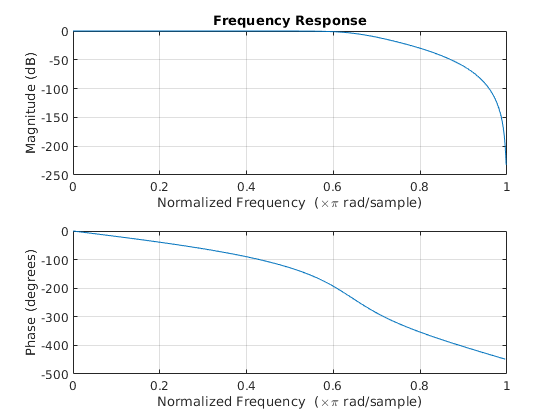
\includegraphics[scale=0.8]{butter.png}
        \caption{Frequency response of Butterworth lowpass filter}
    \end{figure}

    \item[2.] Design a highpass \textbf{Chebyshev} filter:
    \begin{itemize}
        \item two orders: 2, 16
        \item cutoff frequency: 2 rad/s
        \item sampling period: 0.2 s
        \item passband rippling: 3 dB
    \end{itemize}
    \[f_c = \frac{\Omega_c}{2\pi} = \frac{1}{\pi}\]
    \[f_s = \frac{1}{T_s} = 5 Hz\]
    \[\Omega_c(normalized) = \frac{f_c}{f} = 0.127 \]
    We can create the filter using the \textbf{cheby1} function and argument ``high'' to create a highpass filter.\\
    Observing the following graph, we can see that the \(2^{nd}\) order filter has a more gradual ascent (wider transition band) than the \(16^{th}\)
    order one. That means the \(2^{nd}\) order filter is closer to the ideal filter. The \(16^{th}\) order filter has more rippling.
    \begin{figure}[H]
        \centering
        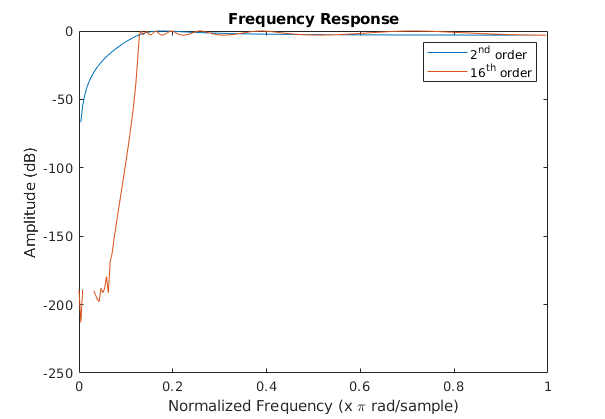
\includegraphics[scale=0.8]{cheby.png}
        \caption{Frequency response of Chebyshev lowpass filter}
    \end{figure}
    \item[3.] Applications of filtering
    \begin{enumerate}
        \item[a.] Apply the \textbf{Butterworth} lowpass filter created in 1.\ onto the following signal:
        \[x(t) = 1 + \cos(1000t) + \cos(16000t) + \cos(30000t)\]
        \[f_1 = \frac{1000}{2\pi} \approx 159\ Hz\]
        \[f_2 = \frac{16000}{2\pi} \approx 2546\ Hz\]
        \[f_3 = \frac{30000}{2\pi} \approx 4774\ Hz\]
        \[f_{Nyq} = 2f_{\max} = 2 \cdot 4774 = 9548\ Hz\]
        \begin{enumerate}
            \item[i.] Sample 500 points using \(f_s = 10 KHz\) as a sampling frequency and create \(x[n]\)
            (No aliasing because \(f_s \geq f_{Nyq}\))
            \item[ii.] Take the Fourier Transform of \(x[n]\) to visualize the frequencies that make up \(x[n]\)
            \item[iii.] Use MATLAB's \textbf{filter} function to apply the filer onto a signal
            \item[iv.] Take the Fourier Transform of the filtered signal to visualize the filtered out frequencies.
            \item[v.] Since the Cutoff frequency is \(4\ KHz\) any frequencies higher should be filtered out.
        \end{enumerate}
        \begin{figure}[H]
            \centering
            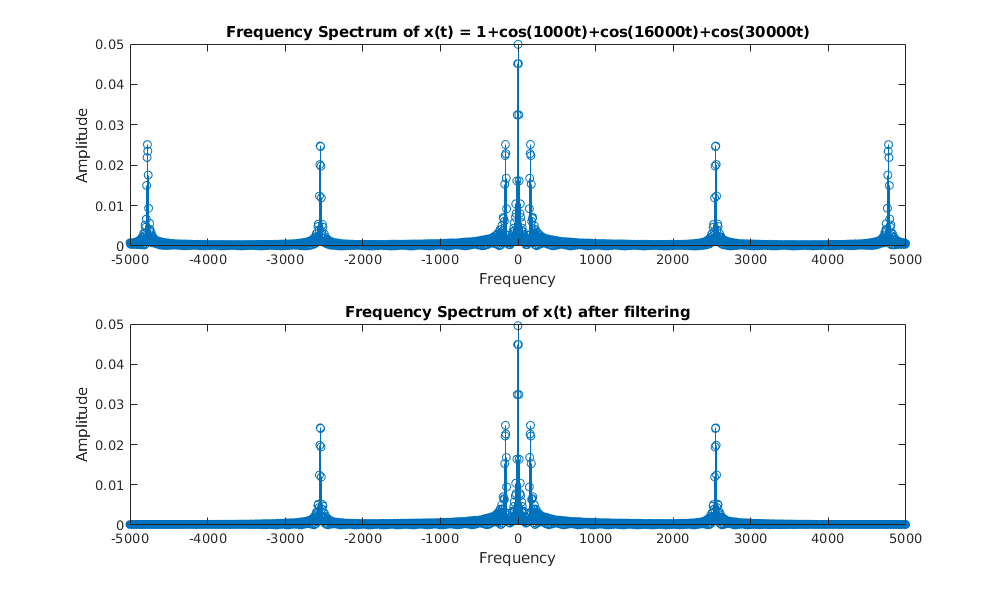
\includegraphics[scale=0.604]{lowpass_app.png}
            \caption{Frequency spectrum before and after filtering}
        \end{figure}
        Indeed we can see that \(f_3 = 4774 Hz\) has been filtered out while the rest of the signal remains intact.
        \item[b.] Apply the \textbf{Chebyshev} highpass filter created in 2.\ onto the following signal:
        \[x(t) = 1 + \cos(1.5t) + \cos(5t)\]
        \[f_1 = \frac{1.5}{2\pi} \approx 0.238\ Hz\]
        \[f_2 = \frac{5}{2\pi} \approx 0.795\ Hz\]
        \[f_c = 0.318\ Hz\]
        The same rules apply for this signal as well. Just as above, Fourier Transform the signal and the use the filter function.
        Observing the following graph we can see that the low frequencies have been filtered out.
        \begin{figure}[H]
            \centering
            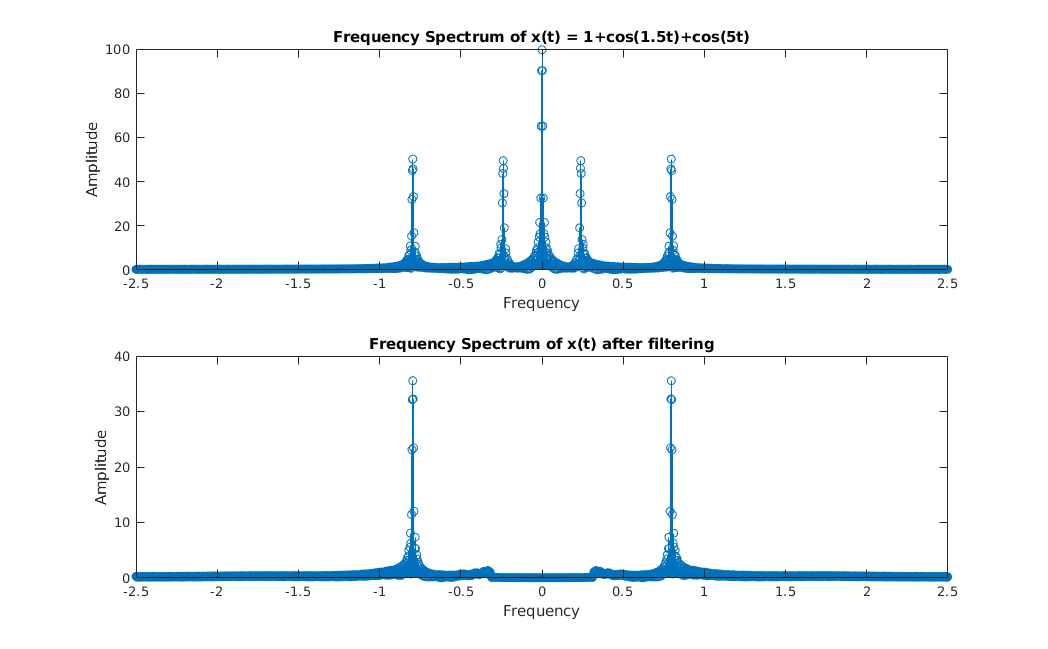
\includegraphics[scale=0.5]{highpass_app.png}
            \caption{Frequency spectrum before and after filtering}
        \end{figure}
    \end{enumerate}
    \item[4.] Design an FIR filter:
    \[\Omega_c = 0.5\pi \]
    \[F_s = 0.1 KHz\]
    With lengths:
    \[N = 21,41\qquad (Hamming, Hanning)\]
    \begin{figure}[H]
        \centering
        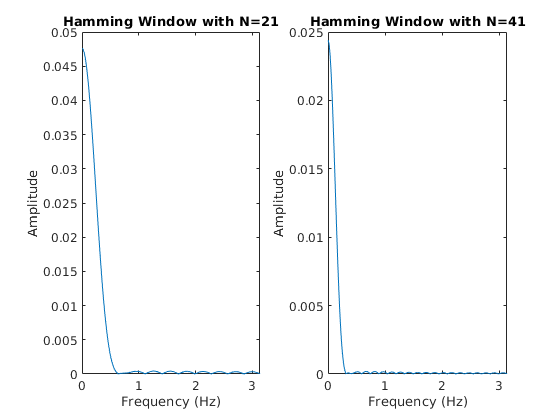
\includegraphics[scale=0.7]{hamming_wins.png}
        \caption{Hamming Windows}
    \end{figure}
    \begin{figure}[H]
        \centering
        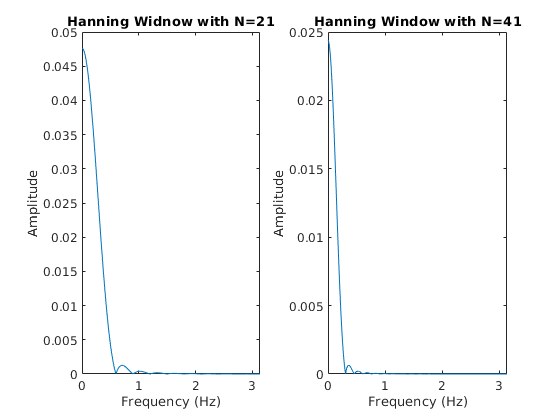
\includegraphics[scale=0.7]{hanning_wins.png}
        \caption{Hanning Windows}
    \end{figure}
    \begin{itemize}
        \item The bigger the window length, the narrower the transition (steeper) band and significally less rippling, 
        thus increasing the window length we can achieve a more effective filter.
        \item The hanning window has an even more stepper transition band and less ripling so it's more effective.
        \item The above differences are the result of the slight difference of their coefficients in their respective equations.
    \end{itemize}
    \pagebreak
    Applying the above mentioned windows onto:
    \[x(t) = \sin(15t) + 0.25\sin(200t),\qquad F_s = 100Hz\]
    \begin{figure}[H]
        \centering
        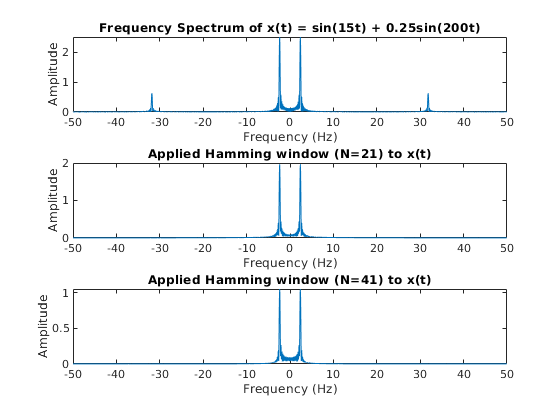
\includegraphics[scale=0.8]{hamm_sig.png}
        \caption{Applied Hamming windows onto \(x(t)\)}
    \end{figure}
    \begin{figure}[H]
        \centering
        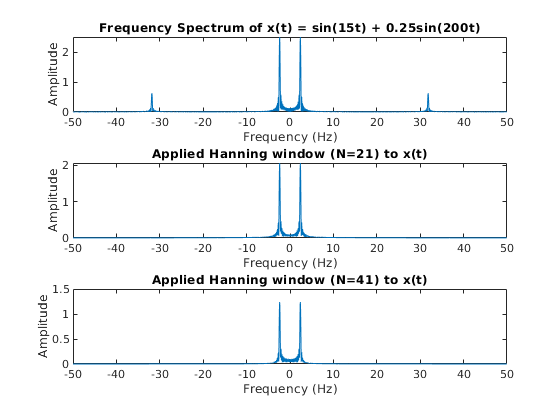
\includegraphics[scale=0.8]{hann_sig.png}
        \caption{Applied Hanning windows onto \(x(t)\)}
    \end{figure}
    \begin{itemize}
        \item The windows with length 41 clip the amplitude more than their counterparts. This is due to the fact that a window's 
        attenuation increases proportional to their length (and ultimately to their band length).
        \item The Hanning window clips reduces the amplitude even more than the Hamming (in both lengths) due to its abrupt transition band.
    \end{itemize}
    Changing the sampling frequency \(F_s\) to \(50 Hz\):
    \begin{figure}[H]
        \centering
        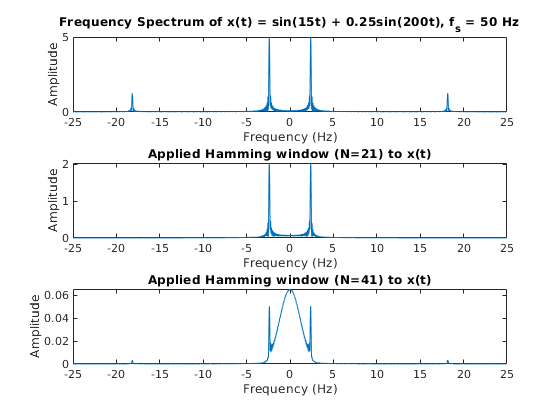
\includegraphics[scale=0.9]{hamm_sig_50.png}
        \caption{Applied Hamming windows onto \(x(t), F_s = 50Hz\)}
    \end{figure}
    \begin{figure}[H]
        \centering
        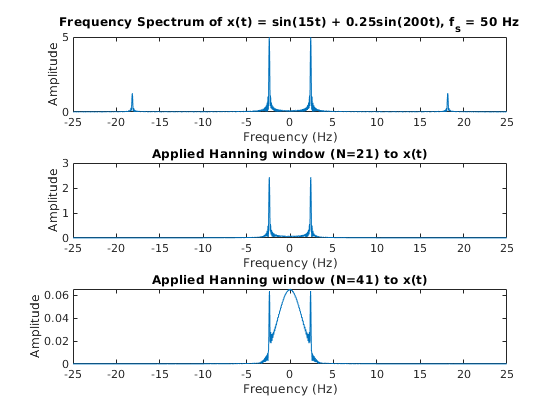
\includegraphics[scale=0.9]{hann_sig_50.png}
        \caption{Applied Hanning windows onto \(x(t), F_s = 50Hz\) }
    \end{figure}
    Chaning the sampling frequency to \(f_s = 50Hz\) creates the phenomenon of aliasing:
    \[f_{\max} = \frac{200}{2\pi} = 31.83 Hz \Rightarrow f_{Nyq} \ge 2f_{\max} = 63.66Hz\]
    As confirmed by the artifacts created.
\end{enumerate}
\end{document}